\documentclass[openany]{book}
\usepackage{graphicx}
\usepackage{mdframed}
\usepackage{tikz}
\usetikzlibrary{calc}
\usepackage{listings}
\usepackage{float}
\usepackage{bbm}
\usepackage{enumitem}
\usepackage{blindtext}
\usepackage{mathtools}
\usepackage{amsmath,amsthm,amssymb}
\usepackage[margin=1in]{geometry}
\usepackage[most]{tcolorbox}
\usepackage{xcolor}
\definecolor{defcolor}{HTML}{D9EAF7}
\definecolor{thmcolor}{HTML}{E8DDF0}
\definecolor{corcolor}{HTML}{EFE3F7}
\definecolor{axcolor}{HTML}{FFF4D6}
\definecolor{conjcolor}{HTML}{FBE4E6}
% ------------------------------------------
% Counter: chapter.section.number
% ------------------------------------------
\renewcommand{\thesection}{\arabic{section}}
\newcounter{mathbox}[section]
\renewcommand{\themathbox}{\thechapter.\thesection.\arabic{mathbox}}

% ------------------------------------------
% Base style for all boxes
% ------------------------------------------
\tcbset{
  mymathbox/.style={
    enhanced,
    breakable,
    left=2mm,right=2mm,top=1mm,bottom=1mm,
    colback=#1!6,
    colframe=#1!60!black,
    fonttitle=\bfseries,
    coltitle=black,
    boxrule=1pt,
    arc=2mm,
    outer arc=2mm,
    before skip=10pt,
    after skip=10pt,
  }
}

% ------------------------------------------
% Definition
% ------------------------------------------
\newenvironment{definition}[1][]{
  \refstepcounter{mathbox}%
  \begin{tcolorbox}[
    mymathbox=defcolor,
    title={Definition~\themathbox\if\relax\detokenize{#1}\relax\else\ (#1)\fi}
  ]
}{
  \end{tcolorbox}
}

% ------------------------------------------
% Theorem
% ------------------------------------------
\newenvironment{theorem}[1][]{
  \refstepcounter{mathbox}%
  \begin{tcolorbox}[
    mymathbox=thmcolor,
    title={Theorem~\themathbox\if\relax\detokenize{#1}\relax\else\ (#1)\fi}
  ]
}{
  \end{tcolorbox}
}

% ------------------------------------------
% Lemma
% ------------------------------------------
\newenvironment{lemma}[1][]{
  \refstepcounter{mathbox}%
  \begin{tcolorbox}[
    mymathbox=thmcolor,
    title={Lemma~\themathbox\if\relax\detokenize{#1}\relax\else\ (#1)\fi}
  ]
}{
  \end{tcolorbox}
}

% ------------------------------------------
% Proposition
% ------------------------------------------
\newenvironment{proposition}[1][]{
  \refstepcounter{mathbox}%
  \begin{tcolorbox}[
    mymathbox=thmcolor,
    title={Proposition~\themathbox\if\relax\detokenize{#1}\relax\else\ (#1)\fi}
  ]
}{
  \end{tcolorbox}
}

% ------------------------------------------
% Corollary
% ------------------------------------------
\newenvironment{corollary}[1][]{
  \refstepcounter{mathbox}%
  \begin{tcolorbox}[
    mymathbox=corcolor,
    title={Corollary~\themathbox\if\relax\detokenize{#1}\relax\else\ (#1)\fi}
  ]
}{
  \end{tcolorbox}
}

% ------------------------------------------
% Axiom
% ------------------------------------------
\newenvironment{axiom}[1][]{
  \refstepcounter{mathbox}%
  \begin{tcolorbox}[
    mymathbox=axcolor,
    title={Axiom~\themathbox\if\relax\detokenize{#1}\relax\else\ (#1)\fi}
  ]
}{
  \end{tcolorbox}
}

% ------------------------------------------
% Conjecture
% ------------------------------------------
\newenvironment{conjecture}[1][]{
  \refstepcounter{mathbox}%
  \begin{tcolorbox}[
    mymathbox=conjcolor,
    title={Conjecture~\themathbox\if\relax\detokenize{#1}\relax\else\ (#1)\fi}
  ]
}{
  \end{tcolorbox}
}

\begin{document}

\begin{titlepage}
   \begin{center}
       \vspace*{1cm}

       \textbf{MATH*RG*4370 Geometry Lecture Notes}

       \vspace{0.8cm}

        \text{Selected topics loosely based on} \textit{The Four Pillars of Geometry} \text{by Dr. John Stillwell} \text{and} \textit{Differential Geometry of Curves and Surfaces} \text{by Dr. Kristopher Tapp}
        
       \vspace{0.5cm}

       \text{Notes adapted by Finn Steinke}


       \vfill
            
       
            
       \vspace{0.8cm}
     
       \includegraphics[width=0.2\textwidth]{IMG_0633.png}
            
       Department of Mathematics and Statistics\\
       University of Guelph\\
       Canada\\
       \today
            
   \end{center}
\end{titlepage}


\setcounter{chapter}{-1}
\chapter{Foundational Geometry}
To begin, we must make ourselves comfortable with certain undefinable notions:
\begin{enumerate}[label=(\roman*)]
    \item points,
    \item lines (curves),
    \item angles,
    \item planes (surfaces),
    \item distances,
\end{enumerate}
among others. We cannot define these without raising more questions, so we must simply use them with a certain level of ignorance. These will be the fundamental tools of our study of geometry.\\
\indent It is interesting to note that (v) will become especially important to us, as even the word "geometry" hints at. The word comes from two Greek primitives ("ge" and "metron") that would directly translate to "earth-measurement". Geometry studies spaces and associated properties that can be measured, such as the aforementioned distances. It is also entirely built on relationships between objects and spaces. Even the way many of us exist relies on some intuitive primitives of "geometry" - many of us use our eyes to collect some semblance of reality, and we live in what can best be described as a "four-dimensional" spacetime. For this reason, the branch of geometry has been the subject of study for ages and is still extremely important in pure mathematics, though often disguised.\\
\indent In this section, we will go through two major branches of geometry, those being synthetic geometry and analytic geometry. It is notable that modern geometry is often extensively studied in conjunction with topology, algebra, analysis, and/or combinatorics. This makes the subject an important stepping stone to most modern mathematical questions, even if they don't seem directly tied to any "physically-realizable" space.

\section{Euclidean Geometry}
Let $\mathbb{R}^{2}$ denote the plane, which we will imagine accepting axiomatically, as we will forego our now typical habit of assigning numbers to points on the plane. Euclidean geometry is formed from Euclid's five postulates.\\

\begin{axiom}
    \textit{We assume the following five postulates to be true for the plane $\mathbb{R}^{2}$:}
    \begin{enumerate}[label=(\roman*)]
        \item \textit{Between two points, we can draw a line.}
        \item \textit{We can indefinitely extend any line.}
        \item \textit{We can draw a circle around any point (called a centre) using a line as a reference (called the radius).}
        \item \textit{All right angles are equal.}
        \item \textit{If any line which crosses two lines makes the interior angles on one side less than two right angles, then the two lines crossed, when extended indefinitely, will cross on the side on which the angle sum is less than two right angles.}
    \end{enumerate}
\end{axiom}

\indent We will only discuss postulates (i), (ii), and (iii) for now, as the notion of an angle as not yet been made precise using points and lines, and postulate (v) was originally a very controversial one; a story for another time.\\
\indent To draw these lines and circles, we use what is called straightedge and compass construction.\\

\begin{definition}
    A \textbf{straightedge and compass construction} is a procedure for producing (drawing) points, lines, and circles in the Euclidean plane $\mathbb{R}^{2}$, beginning from a given finite set of initial points, using only the following operations:
    \begin{enumerate}[label=(\roman*)]
        \item Drawing the unique line passing through any two distinct constructed points.
        \item Drawing the circle with any constructed point as its centre and with radius drawn between any two constructed points.
        \item Taking as new constructed points any intersections of previously constructed lines and circles.
    \end{enumerate}
\end{definition}


\indent With this notion of construction, we have successfully developed an approach to geometry on $\mathbb{R}^{2}$ without the need for distances. We can now gain a visual intuition for how we represent certain of the aforementioned "undefinable" notions. For example, while an angle itself has no definition, it is visually represented as the "space between" two lines that meet at a point. Given two points $A, B$ and using straightedge and compass construction, we draw two circles centred at $A$ and $B$ respectively, and find that they share two points, one of which we call $C$. From this point $C$, we can produce lines back to the centres, where we find there is now an angle, which we denote $\angle ACB$.
\begin{center}
    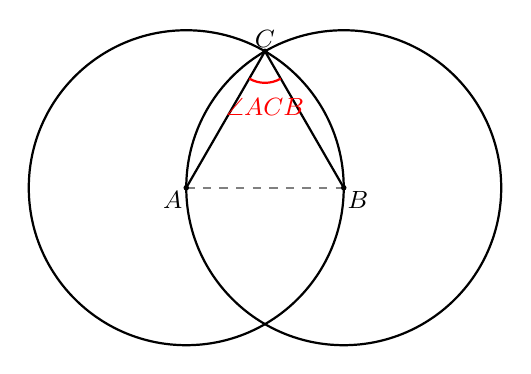
\begin{tikzpicture}[scale=1.0, thick,
        every node/.style={font=\small, inner sep=1pt}]
        % Define points
        \coordinate (A) at (0,0);
        \coordinate (B) at (2,0);
        \coordinate (C) at (1,{sqrt(3)}); % top intersection point
    
        % Draw circles centered at A and B with radius AB = 2
        \draw (A) circle (2);
        \draw (B) circle (2);
    
        % Draw baseline and triangle sides
        \draw[gray, dashed] (A) -- (B);
        \draw (A) -- (C);
        \draw (B) -- (C);
    
        % Mark points
        \fill (A) circle(1pt) node[below left] {$A$};
        \fill (B) circle(1pt) node[below right] {$B$};
        \fill (C) circle(1pt) node[above] {$C$};
    
        % Draw small red angle at C (between CA and CB)
        \draw[red] ($(C)+(-120:0.4)$) arc[start angle=-120, end angle=-60, radius=0.4];
        \node[red] at ($(C)+(-90:0.7)$) {$\angle ACB$};
    \end{tikzpicture}
\end{center}

\indent In fact, we can recover the definition of a right angle here too, by producing a line from $A$ to $B$, and from $C$ to the other point shared between two circles, we call it $D$. These two lines will meet at a point, which we call $E$, and from here we can intuitively see that $\angle AEC$ is a right angle.
\begin{center}
    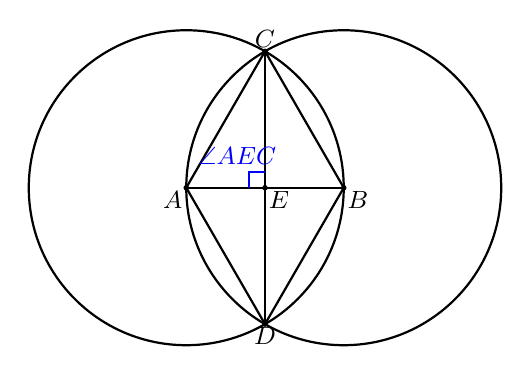
\begin{tikzpicture}[scale=1.0, thick,
        every node/.style={font=\small, inner sep=1pt}]
        % Points
        \coordinate (A) at (0,0);
        \coordinate (B) at (2,0);
        \coordinate (C) at (1,{sqrt(3)});   % top intersection
        \coordinate (D) at (1,-{sqrt(3)});  % bottom intersection
    
        % Draw circles
        \draw (A) circle (2);
        \draw (B) circle (2);
    
        % Draw baseline and triangle/construction lines
        \draw (A) -- (B);         % solid baseline
        \draw (A) -- (C);
        \draw (B) -- (C);
        \draw (A) -- (D);
        \draw (B) -- (D);
        \draw (C) -- (D);         % line connecting intersections
    
        % Mark points
        \fill (A) circle(1pt) node[below left] {$A$};
        \fill (B) circle(1pt) node[below right] {$B$};
        \fill (C) circle(1pt) node[above] {$C$};
        \fill (D) circle(1pt) node[below] {$D$};
    
        % Intersection E (schematic for right angle)
        \coordinate (E) at (1,0); 
        \fill (E) circle(1pt) node[below right] {$E$};
    
        % Draw small blue right angle at E
        \draw[blue] ($(E)+(-0.2,0)$) -- ++(0,0.2) -- ++(0.2,0);
        \node[blue] at ($(E)+(-0.35,0.4)$) {$\angle AEC$};
    \end{tikzpicture}
\end{center}

\indent It is now that we should begin a digression on what exactly equality entails in our "synthetic" constructions. To do this, we will begin to restate our notions of synthetic geometry with modern rigor, using Tarski's axioms for synthetic geometry.\\

\begin{definition}
    Let $\mathcal{E} = (X, B, \cong)$ be an \textbf{abstract geometry}, where $X$ is some non-empty set of points, $B\subseteq X^{3}$ is a betweenness relation, and $\cong\:\subseteq X^{4}$ is a congruence relation.
\end{definition}

Let's discuss those relations in depth, and where we can get our other "undefinables" from in this system.\\

\begin{definition}
    A \textbf{betweenness relation} $B$ is a relation given by
    \[B = \big\{(A,C,D)\in X\!\times\! X\!\times\!  X\big\},\]
    such that it satisfies:
    \begin{enumerate}[label=(\roman*)]
        \item If $B(A,B,C)$, then $B(C,B,A)$,
        \item If $B(A,B,C)$, then $A\neq B \neq C$,
        \item If $B(A,B,C)$ and $B(A,C,D)$, then $B(A,B,D)$,
        \item For all $A, B\in X$ where $A\neq B$, there exists $C\in X$ such that $B(A,B,C)$.
    \end{enumerate}
\end{definition}
With this, we can formally construct our previously undefinable terms, such as a line segment, where
\begin{align*}
    \overline{AC} &\coloneq\big\{B\in X\:|\:B(A,B,C)\big\} \cup \{A, C\}.
\end{align*}
For clarity, we usually just write $AC$ to denote a line segment, \textit{i}.\textit{e}., $AC\coloneq \overline{AC}$. We can extend our line segments indefinitely on one side, without loss of generality, to get a ray, where
\begin{align*}
    \overrightarrow{AC} &\coloneq\big\{B\in X\:|\:B(A,B,C),\text{ or } B(A,C,B)\big\} \cup \{A, C\}.
\end{align*}
Extending once more we can get a line, where
\begin{align*}
    \overleftrightarrow{AC} &\coloneq\big\{B\in X\:|\:B(A,B,C),\text{ or } B(A,C,B),\text{ or } B(B,A,C\big\} \cup \{A, C\}.
\end{align*}
For a more complex construction, consider the triangle, where
\begin{align*}
    \triangle ABC\coloneq AB\cup BC\cup AC,
\end{align*}
where in the case that $B(A,B,C), B(A,C,B), B(B,A,C)$, we have the degenerate "triangle", $\tilde{\triangle}ABC = AC$. Now, we can define our second relation in our abstract geometry.\\

\begin{definition}
    A \textbf{congruence relation} $\cong$ is a relation given by
    \[\cong\:=\{\big((A,B),(C,D)\big)\in (X\times X)\times (X\times X)\},\]
    such that it satisfies
    \begin{enumerate}[label=(\roman*)]
        \item For all $A,B\in X$, $AB\cong BA$,
        \item For all $A,B,\dots, F\in X$, if $AB\cong CD$ and $AB\cong EF$, then $CD \cong EF$,
        \item For all $A,B,C,Q\in X$, there exists some $P\in X$ such that $B(Q, A, P)$ and $AQ \cong BC$,
        \item For all $A,B,C,D, A', B', C', D'\in X$, if $AB\cong A'B'$, $BC\cong B'C'$, $AD\cong A'D'$, $BD\cong B'D'$, $B(A,B,C)$, and $B(A',B',C')$, then $CD\cong C'D'$.
    \end{enumerate}
\end{definition}
This relation allows us to create even more basic constructions, like a circle for example:
\begin{align*}
    \mathcal{C}(OA) \coloneq \{B\in X\:|\:OA\cong OB\},
\end{align*}
where $O$ represents the centre point of the circle. We can continue our discussion by introducing angles, an absolutely fundamental tool moving forward.\\

\begin{definition}
    An \textbf{angle} is given by the ordered pair
    \[\angle ABC \coloneq \big(\overrightarrow{BA}, \overrightarrow{BC}\big),\]
    where $B$ is known as the vertex of the angle. Angles can be congruent, where we denote
    \[\angle ABC \cong \angle A'B'C',\]
    if there exist points $D\in\overrightarrow{BA}$, $E\in\overrightarrow{BC}$ and $D'
    \in\overrightarrow{B'C'}$, $E'\in\overrightarrow{B'C'}$ such that $BD \cong B'D'$, $BE \cong B'E'$, and $DE\cong D'E'$.
\end{definition}


\section{Analytic Geometry}
To solidify our understanding of analytic geometry, we will revisit a few concepts in linear algebra.\\

\begin{definition}
    A \textbf{vector space} $V$ is a set over a field $\mathbbm{k}$ with the standard field operations, in addition to addition and scalar multiplication of vector space elements (called vectors).
\end{definition}

\begin{definition}
    An \textbf{inner product space} is an ordered pair $\big(V, \langle\cdot,\cdot\rangle\big)$, where $V$ is a vector space and \\$\langle\cdot,\cdot\rangle:V\times V\to\mathbbm{k}$ is a map known as the inner product.
\end{definition}

\indent From this inner product space, we can automatically find a norm, where $||\mathbf{x}|| = \sqrt{\langle\mathbf{x},\mathbf{x}\rangle}$, with $\mathbf{x}\in V$. In fact, this norm induces a metric, which we know is given by
\begin{align*}
    d(\mathbf{x},\mathbf{y}) &= ||\mathbf{x}-\mathbf{y}||,
\end{align*}
where $\mathbf{x},\mathbf{y}\in V$. This metric is extremely useful, as it will give us a notion of distance on our space.\\

\indent Now to define the space with which we would like to work on. We know from our physical intuition that Euclid's constructions are certainly valid, but they don't cover everything. For example, lets say we wished to "slide" a given triangle a certain small distance. Sure, we could go about constructing a very intricate method of reproducing a triangle congruent to the first at varying small distances from the first, but the question remains - are all distances covered, i.e., is our transformation (slide) "smooth"? We can talk more about theses smooth maps and transformations as we discuss differential geometry, but we gain a basic understanding through the following discussion. We claim that the majority of distances we are able to slide such a triangle are missing/undefined. A popular example of such a distance could be the number $e$. Bottom line is, we need to define all of these kinds of numbers.\\

\indent We know from results in analysis that the space $\big(\mathbb{Q},||\cdot||\big)$ is missing points. We might, rightfully, assume that the replacing $\mathbb{Q}$ with the constructible or even the algebraic numbers could yield a more "full" space without any missing points, however, this is not the case. From analysis, we know that a complete space is one where every Cauchy sequence converges in the space itself, and there exist Cauchy sequences in the constructible numbers that converge outside of the constructible numbers, such as the rational sequence
\begin{align*}
    (3, 3.1, 3.14, 3.141, \dots),
\end{align*}
where we know that the above converges to $\pi$. In fact, the completion of the constructible numbers is $\mathbb{R}$, and so topologically, $\big(\mathbb{R}^{2},||\cdot||\big)$ is said to be complete with respect to any choice of norm. Using ideas regarding proportionality from our discussions of Euclidean geometry, we can now define a familiar quantity:\\

\indent Let $O = (0,0)$ be defined as the origin, and let us distinguish important lines, which we call axes. To define our points given a vector space idea, we consider the isomorphism $T:\mathbb{R}^{2} \to \mathbb{R}^{2}$, where $P\mapsto OP$, where each vector $OP = (x-0, y-0) = (x,y)$. Then, the point $P$ corresponds to the coordinate vector $(x,y)$. This allows us to reach any point, simply by changing the values of $x,y\in\mathbb{R}$.\\

\begin{definition}
    Given our synthetic ideas, we know that $|AB|$ denotes distance. If we give each length a \textbf{direction}, we imagine drawing $PQ$ from point $P$ to point $Q$, so if $P = (x_{1},y_{1})$ and $Q = (x_{2},y_{2})$, then we know that $d(Q, P)$ will remain positive, but we can give each component a signed length, where
\begin{align*}
    y_{2} -y_{1},\quad \text{ and }\quad x_{2}-x_{1}.
\end{align*}
\end{definition}
\indent In fact, we can extend this idea of signed magnitudes further to our proportionality, where $\dfrac{|OC|}{|OA|} = \dfrac{|OD|}{|OB|} = |a|$, where the right-hand $|\cdot|$ denotes the absolute value on $\mathbb{R}$. This quantity $a$ becomes signed when we consider the signed distances of each of the line segments, and hence is called the slope of both lines. In fact, for any line segment, ray, or line, we can choose two points and use our signed component lengths to get
\begin{align*}
    a = \frac{y_{2}-y_{1}}{x_{2}-x_{1}},
\end{align*}
a very comfortable result for us indeed.\\

\indent It is now that we make the above discussion explicit in an analytic and algebraic way. 
The central idea of analytic geometry is that geometric objects can be encoded by numbers, 
and that collections of numbers can be manipulated algebraically. Historically, this idea 
was introduced by René Descartes and Pierre de Fermat.

\begin{definition}
    An \textbf{$n$-tuple} is an ordered list of $n$ real numbers, written
    \[
        (x_1, x_2, \dots, x_n),
    \]
    where each $x_i \in \mathbb{R}$.
\end{definition}

We refer to $x_i$ as the \textbf{$i$-th coordinate} of the $n$-tuple. 
The order of the entries is essential: in general,
\[
(x_1, x_2, \dots, x_n) \neq (x_{\sigma(1)}, x_{\sigma(2)}, \dots, x_{\sigma(n)})
\]
for a nontrivial permutation $\sigma$.

\medskip

\indent At first glance, an $n$-tuple is simply a collection of numbers. 
However, the crucial observation of analytic geometry is that such tuples can be interpreted 
as \emph{vectors}, and hence inherit the algebraic structure of a vector space.

\begin{definition}
    The vector space $\mathbb{R}^n$ is the set of all $n$-tuples of real numbers,
    \[
        \mathbb{R}^n := \{(x_1, \dots, x_n) \mid x_i \in \mathbb{R}\},
    \]
    equipped with componentwise addition and scalar multiplication.
\end{definition}

Under this definition, each $n$-tuple determines a unique vector in $\mathbb{R}^n$, and 
conversely, every vector in $\mathbb{R}^n$ is uniquely determined by its coordinates. 
Thus, there is a natural identification
\[
    (x_1, \dots, x_n) \;\longleftrightarrow\; x_1 \mathbf{e}_1 + \cdots + x_n \mathbf{e}_n,
\]
where $\{\mathbf{e}_1, \dots, \mathbf{e}_n\}$ denotes the standard basis of $\mathbb{R}^n$.

\medskip

\indent In particular, the plane studied earlier corresponds to $\mathbb{R}^2$, where each point 
$P = (x,y)$ may be viewed either as a geometric location or as a vector based at the origin. 
This identification allows us to translate geometric questions—such as distance, direction, 
and slope—into algebraic ones involving vectors, norms, and inner products.

\medskip

\indent This correspondence between geometry and algebra is the foundation of analytic geometry, 
and it will allow us to generalize classical Euclidean constructions to higher dimensions and 
more abstract settings.

\indent We observe that any geometric construction ultimately produces lengths, based on our definition of norm, for a normed vector space. By fixing a unit length, all other constructible lengths may be interpreted as real numbers. 
The fundamental question then becomes: \emph{which real numbers can arise from straightedge-and-compass constructions?}

\indent From an algebraic perspective, we start with the field of rational numbers $\mathbb{Q}$, which corresponds to the lengths obtainable by repeated addition, subtraction, multiplication, and division of the unit segment. 
Each new construction step introduces the intersection of lines and circles, operations that algebraically correspond to solving linear and quadratic equations.

\begin{definition}
    A real number $\alpha \in \mathbb{R}$ is called \textbf{constructible} if there exists a finite tower of field extensions
    \[
        \mathbb{Q} = K_0 \subset K_1 \subset \cdots \subset K_n
    \]
    such that $\alpha \in K_n$ and each extension $K_{i+1}/K_i$ has degree $[K_{i+1} : K_i] = 2$.
\end{definition}

\indent The set of all constructible numbers forms a field, denoted by $\mathbb{Q}_{\mathrm{con}}$, and is the smallest subfield of $\mathbb{R}$ containing $\mathbb{Q}$ that is closed under taking square roots of positive elements.

\indent Equivalently, a real number is constructible if and only if it can be obtained from $\mathbb{Q}$ by finitely many applications of the operation
\[
    x \mapsto \sqrt{x}, \quad x > 0,
\]
together with the usual field operations.

\indent This characterization immediately implies that every constructible number is algebraic over $\mathbb{Q}$, and that its minimal polynomial has degree a power of two. 
Consequently, many familiar numbers—such as $\pi$ and $e$—are not constructible. We recall the definition of algebraic numbers now.

\begin{definition}
    A real number $\alpha \in \mathbb{R}$ is called \textbf{algebraic over $\mathbb{Q}$} if there exists a nonzero polynomial
    \[
        p(x) = a_n x^n + \cdots + a_1 x + a_0 \in \mathbb{Q}[x]
    \]
    such that $p(\alpha) = 0$.
\end{definition}

\indent If no such polynomial exists, $\alpha$ is called \textbf{transcendental}. 
We denote by $\overline{\mathbb{Q}}\cap\mathbb{R}$ the set of all algebraic numbers (in $\mathbb{R}$).

\indent The algebraic numbers form a field containing $\mathbb{Q}$ and are closed under addition, subtraction, multiplication, and division. 
Moreover, every algebraic number $\alpha$ has a unique monic polynomial of minimal degree in $\mathbb{Q}[x]$ for which $\alpha$ is a root; this polynomial is called the \textbf{minimal polynomial} of $\alpha$, and its degree is denoted $[\mathbb{Q}(\alpha) : \mathbb{Q}]$.

\indent Many familiar numbers are algebraic. For example,
\[
    \sqrt{2} \text{ is algebraic since } x^2 - 2 = 0,
\]
and more generally, any root of a polynomial equation with rational coefficients is algebraic. 
However, not all real numbers are algebraic: classical results show that numbers such as $\pi$ and $e$ are transcendental.

\indent This distinction allows us to place constructible numbers within a broader algebraic framework. 
As we shall see, every constructible number is algebraic over $\mathbb{Q}$, but not every algebraic number is constructible. 
The difference lies in the degrees of the corresponding field extensions.

\indent These notions fit into the following chain of inclusions:
\[
    \mathbb{Q}
    \;\subset\;
    \mathbb{Q}_{\mathrm{con}}
    \;\subset\;
    \overline{\mathbb{Q}}\cap\mathbb{R}
    \;\subset\;
    \mathbb{R}.
\]
\indent From a geometric viewpoint, each enlargement of $\mathbb{Q}$ corresponds to allowing 
new constructions or operations. From an analytic viewpoint, however, even the field of algebraic 
numbers is incomplete as a metric space, motivating the passage to the real numbers $\mathbb{R}$ 
as a completion. Although classical geometry leads naturally to algebraic and constructible field extensions of $\mathbb{Q}$, it is only upon completing these fields to $\mathbb{R}$ that distances vary continuously and geometric motion becomes well-defined, thereby requiring analysis and motivating the term \textit{analytic} geometry. 

\indent Our prior understanding of vectors and coordinate geometry is now made immediately clear. We now have access to all of $\mathbb{R}^{n}$, which allows us to \textbf{(CONTINUE)}\\




\textbf{(ISOMETRY)}



\chapter{Elementary Differential Geometry}

\section{Curves}
\begin{definition}
    Given a metric space $(X, d)$ and some interval $I\subseteq\mathbb{R}$, a \textbf{curve} is a continuous map $\gamma:I\to X$.
\end{definition}
Typically, we identify endpoints, and so $I =[a,b]$, with $a \leq b$ (called an arc). We recall that a continuous map requires that any open image $U\subset X$ must have an open preimage $\gamma^{-1}(U)\subset I$. Hence, for any homeomorphism $\phi:I \to I$, we know that $\gamma\circ\phi:I \to X$, and so $\gamma\circ\phi$ is also a curve (recall that homeomorphisms must be bijective and continuous). We will review some functional basics. We can classify functions based on their "smoothness", where we know that for any space $X$,
\begin{align*}
    C^{0}(X)\supset C^{1}(X) \supset C^{2}(X) \supset \cdots \supset C^{k}(X) \supset\cdots \supset C^{\infty}(X)\supset\cdots \supset C^{\omega}(X).
\end{align*}
Since $\gamma$ is simply a function of $t\in I$, we know that any curve can be denoted as "sufficiently smooth", which is especially useful when observing certain properties of curves in smooth spaces. We will return to these ideas shortly. We first define the notion of arc length with a few prerequisites. Recall the following definition.\\

\begin{definition}
    Given a compact real interval $[a,b]\subset\mathbb{R}$, a \textbf{partition of the interval} is a finite strictly monotone increasing sequence $(x_{i})_{i\in\{0\}\cup[n]}\subset[a,b]$ such that $x_{0} = a$ and $x_{n} = b$.
\end{definition}
The partition creates a family of intervals that only overlap at endpoints of the form $\big([x_{i-1}, x_{i}]\big)_{i\in[n]}$. With this construction, we find consider the next definition.\\

\begin{definition}
    Given a metric space $(X,d)$ and a curve $\gamma:[a,b]\to X$, the \textbf{polygonal approximation of the arc length} of a curve $\gamma$ with respect to the partition $\mathcal{P}$ is the map $L:C^{0}(X)\to \mathbb{R}$ defined by
    \begin{align*}
        L(\gamma, \mathcal{P}) =\sum_{i\in[n]}d\big(\gamma(t_{i-1}), \gamma(t_{i})\big).
    \end{align*}
\end{definition}
Extending this, we get the following.\\

\begin{definition}
    Given Given a metric space $(X,d)$ and a curve $\gamma:[a,b]\to X$, the \textbf{arc length} is the map $L:C^{0}(X)\to \mathbb{R}$ is defined by
    \begin{align*}
        L(\gamma) = \sup_{\mathcal{P}}L(\gamma, \mathcal{P}),
    \end{align*}
    where $n$ is variable for each $\mathcal{P}$.
\end{definition}


Consider the normed space $\big(V, ||\cdot||\big)$ with a curve $\gamma:[a,b]\to V$. Then we know that the induced metric gives us a polygonal approximation of the arc length of a curve $\gamma$ with respect to the partition $\mathcal{P}$ is given by
\begin{align*}
    L(\gamma, \mathcal{P}) =\sum_{i\in[n]}\big|\big|\gamma(t_{i})- \gamma(t_{i-1}) \big|\big|,
\end{align*}
with arc length
\begin{align*}
    L(\gamma) = \sup_{\mathcal{P}}L(\gamma, \mathcal{P}).
\end{align*}
With a bit of analytical work, this definition of arc length reminds us of another common notion in analysis. Suppose that $\gamma$ is absolutely continuous on $[a,b]$, where we then know by a corollary of first part of the fundamental theorem of calculus that \textbf{(REVIEW USE OF SUP IN POLY. APP.)}
\begin{align*}
    \gamma(t_{i}) - \gamma(t_{i-1}) = \int\limits_{t_{i-1}}^{t_{i}}\frac{\mathrm{d}\gamma}{\mathrm{d}u}\:\mathrm{d}u,
\end{align*}
where by change of variables the above Bochner integral is well-defined. We will adopt the shorthand $\gamma'(u) = \dfrac{\mathrm{d}\gamma}{\mathrm{d}u}$ for convenience. Then we know that for all $i\in[n]$ we have
\begin{align*}
    \big|\big|\gamma(t_{i}) - \gamma(t_{i-1})\big|\big| &= \Bigg|\Bigg|\int\limits_{t_{i-1}}^{t_{i}}\gamma'(u)\:\mathrm{d}u\:\Bigg|\Bigg|\\
    &\leq \int\limits_{t_{i-1}}^{t_{i}}\big|\big|\gamma'(u)\big|\big|\:\mathrm{d}u.
\end{align*}
Then it follows that
\begin{align*}
    \sum_{i\in[n]}\big|\big|\gamma(t_{i})-\gamma(t_{i-1})\big|\big| &\leq \int\limits_{a}^{b}\big|\big|\gamma'(u)\big|\big|\:\mathrm{d}u\\
    \iff \sup_{\mathcal{P}}\sum_{i\in[n]}\big|\big|\gamma(t_{i})-\gamma(t_{i-1})\big|\big| &\leq \int\limits_{a}^{b}\big|\big|\gamma'(u)\big|\big|\:\mathrm{d}u\\
    \iff L(\gamma) &\leq \int\limits_{a}^{b}\big|\big|\gamma'(u)\big|\big|\:\mathrm{d}u.
\end{align*}
It can additionally be proved using Egorov's theorem and Lebesgue's differentiation theorem that
\begin{align*}
    L(\gamma) &\geq \int\limits_{a}^{b}\big|\big|\gamma'(u)\big|\big|\:\mathrm{d}u,
\end{align*}
and thus we arrive at our final expression for arc length in a normed space
\begin{align*}
    L(\gamma) &= \int\limits_{a}^{b}\big|\big|\gamma'(u)\big|\big|\:\mathrm{d}u,
\end{align*}
where the above integral is a Lebesgue integral, i.e.,
\begin{align*}
    \int\limits_{a}^{b}\big|\big|\gamma'(u)\big|\big|\:\mathrm{d}u &= \int_{[a,b]}\Big|\Big|\dfrac{\mathrm{d}\gamma}{\mathrm{d}u}\Big|\Big|\:\mathrm{d}\lambda(u),
\end{align*}
where $\dfrac{\mathrm{d}\gamma}{\mathrm{d}u}$ is the usual Fréchet derivative.

\textbf{(FRENET-SERRET FRAME)}

\end{document}